\documentclass[11pt,compress,t,notes=noshow, xcolor=table]{beamer}
\usepackage[]{graphicx}\usepackage[]{color}
% maxwidth is the original width if it is less than linewidth
% otherwise use linewidth (to make sure the graphics do not exceed the margin)
\makeatletter
\def\maxwidth{ %
  \ifdim\Gin@nat@width>\linewidth
    \linewidth
  \else
    \Gin@nat@width
  \fi
}
\makeatother

\definecolor{fgcolor}{rgb}{0.345, 0.345, 0.345}
\newcommand{\hlnum}[1]{\textcolor[rgb]{0.686,0.059,0.569}{#1}}%
\newcommand{\hlstr}[1]{\textcolor[rgb]{0.192,0.494,0.8}{#1}}%
\newcommand{\hlcom}[1]{\textcolor[rgb]{0.678,0.584,0.686}{\textit{#1}}}%
\newcommand{\hlopt}[1]{\textcolor[rgb]{0,0,0}{#1}}%
\newcommand{\hlstd}[1]{\textcolor[rgb]{0.345,0.345,0.345}{#1}}%
\newcommand{\hlkwa}[1]{\textcolor[rgb]{0.161,0.373,0.58}{\textbf{#1}}}%
\newcommand{\hlkwb}[1]{\textcolor[rgb]{0.69,0.353,0.396}{#1}}%
\newcommand{\hlkwc}[1]{\textcolor[rgb]{0.333,0.667,0.333}{#1}}%
\newcommand{\hlkwd}[1]{\textcolor[rgb]{0.737,0.353,0.396}{\textbf{#1}}}%
\let\hlipl\hlkwb

\usepackage{framed}
\makeatletter
\newenvironment{kframe}{%
 \def\at@end@of@kframe{}%
 \ifinner\ifhmode%
  \def\at@end@of@kframe{\end{minipage}}%
  \begin{minipage}{\columnwidth}%
 \fi\fi%
 \def\FrameCommand##1{\hskip\@totalleftmargin \hskip-\fboxsep
 \colorbox{shadecolor}{##1}\hskip-\fboxsep
     % There is no \\@totalrightmargin, so:
     \hskip-\linewidth \hskip-\@totalleftmargin \hskip\columnwidth}%
 \MakeFramed {\advance\hsize-\width
   \@totalleftmargin\z@ \linewidth\hsize
   \@setminipage}}%
 {\par\unskip\endMakeFramed%
 \at@end@of@kframe}
\makeatother

\definecolor{shadecolor}{rgb}{.97, .97, .97}
\definecolor{messagecolor}{rgb}{0, 0, 0}
\definecolor{warningcolor}{rgb}{1, 0, 1}
\definecolor{errorcolor}{rgb}{1, 0, 0}
\newenvironment{knitrout}{}{} % an empty environment to be redefined in TeX

\usepackage{alltt}
\newcommand{\SweaveOpts}[1]{}  % do not interfere with LaTeX
\newcommand{\SweaveInput}[1]{} % because they are not real TeX commands
\newcommand{\Sexpr}[1]{}       % will only be parsed by R



\usepackage[english]{babel}
\usepackage[utf8]{inputenc}

\usepackage{dsfont}
\usepackage{verbatim}
\usepackage{amsmath}
\usepackage{amsfonts}
\usepackage{bm}
\usepackage{csquotes}
\usepackage{multirow}
\usepackage{longtable}
\usepackage{booktabs}
\usepackage{enumerate}
\usepackage[absolute,overlay]{textpos}
\usepackage{psfrag}
\usepackage{algorithm}
\usepackage{algpseudocode}
\usepackage{eqnarray}
\usepackage{arydshln}
\usepackage{tabularx}
\usepackage{placeins}
\usepackage{tikz}
\usepackage{setspace}
\usepackage{colortbl}
\usepackage{mathtools}
\usepackage{wrapfig}
\usepackage{bm}
\usetikzlibrary{shapes,arrows,automata,positioning,calc,chains,trees, shadows}
\tikzset{
  %Define standard arrow tip
  >=stealth',
  %Define style for boxes
  punkt/.style={
    rectangle,
    rounded corners,
    draw=black, very thick,
    text width=6.5em,
    minimum height=2em,
    text centered},
  % Define arrow style
  pil/.style={
    ->,
    thick,
    shorten <=2pt,
    shorten >=2pt,}
}
\usepackage{subfig}


% Defines macros and environments

% basic latex stuff
\newcommand{\pkg}[1]{{\fontseries{b}\selectfont #1}} %fontstyle for R packages
\newcommand{\lz}{\vspace{0.5cm}} %vertical space
\newcommand{\dlz}{\vspace{1cm}} %double vertical space
\newcommand{\mat}[1]{ %short pmatrix command
  \begin{pmatrix}
    #1
  \end{pmatrix}
}
\newcommand{\oneliner}[1] % Oneliner for important statements
{\begin{block}{}\begin{center}\begin{Large}#1\end{Large}\end{center}\end{block}}


% 
% basic latex stuff
\newcommand{\pkg}[1]{{\fontseries{b}\selectfont #1}} %fontstyle for R packages
\newcommand{\lz}{\vspace{0.5cm}} %vertical space
\newcommand{\dlz}{\vspace{1cm}} %double vertical space
\newcommand{\mat}[1]{ %short pmatrix command
  \begin{pmatrix}
    #1
  \end{pmatrix}
}
\newcommand{\oneliner}[1] % Oneliner for important statements
{\begin{block}{}\begin{center}\begin{Large}#1\end{Large}\end{center}\end{block}}



%\usetheme{lmu-lecture}
\usepackage{../../style/lmu-lecture}

\let\code=\texttt
\let\proglang=\textsf

\setkeys{Gin}{width=0.9\textwidth}

\title{Introduction to Machine Learning}
% \author{Bernd Bischl, Christoph Molnar, Daniel Schalk, Fabian Scheipl}
\institute{\href{https://compstat-lmu.github.io/lecture_i2ml/}{compstat-lmu.github.io/lecture\_i2ml}}
\date{}

\setbeamertemplate{frametitle}{\expandafter\uppercase\expandafter\insertframetitle}



\begin{document}



% This file loads R packages, configures knitr options and sets preamble.Rnw as parent file
% IF YOU MODIFY THIS, PLZ ALSO MODIFY setup.Rmd ACCORDINGLY...








% Defines macros and environments
% math spaces
\newcommand{\N}{\mathds{N}}                                                 % N, naturals
\newcommand{\Z}{\mathds{Z}}                                                 % Z, integers
\newcommand{\Q}{\mathds{Q}}                                                 % Q, rationals
\newcommand{\R}{\mathds{R}}                                                 % R, reals
\newcommand{\C}{\mathds{C}}                                                 % C, complex
\newcommand{\HS}{\mathcal{H}}                                               % H, hilbertspace
\newcommand{\continuous}{\mathcal{C}}                                       % C, space of continuous functions
\newcommand{\M}{\mathcal{M}} 												% machine numbers
\newcommand{\epsm}{\epsilon_m} 												% maximum error


% basic math stuff
\newcommand{\xt}{\tilde x}													% x tilde
\def\argmax{\mathop{\sf arg\,max}}                                          % argmax
\def\argmin{\mathop{\sf arg\,min}}                                          % argmin
\newcommand{\sign}{\operatorname{sign}}                                     % sign, signum
\newcommand{\I}{\mathbb{I}}                                                 % I, indicator
\newcommand{\order}{\mathcal{O}}                                            % O, order
\newcommand{\fp}[2]{\frac{\partial #1}{\partial #2}}                        % partial derivative
\newcommand{\pd}[2]{\frac{\partial{#1}}{\partial #2}}						% partial derivative

% sums and products
\newcommand{\sumin}{\sum_{i=1}^n}											% summation from i=1 to n
\newcommand{\sumkg}{\sum_{k=1}^g}											% summation from k=1 to g
\newcommand{\prodin}{\prod_{i=1}^n}											% product from i=1 to n
\newcommand{\prodkg}{\prod_{k=1}^g}											% product from k=1 to g

% linear algebra
\newcommand{\one}{\boldsymbol{1}}                                           % 1, unitvector
\newcommand{\id}{\mathrm{I}}                                                % I, identity
\newcommand{\diag}{\operatorname{diag}}                                     % diag, diagonal
\newcommand{\trace}{\operatorname{tr}}                                      % tr, trace
\newcommand{\spn}{\operatorname{span}}                                      % span
\newcommand{\scp}[2]{\left\langle #1, #2 \right\rangle}                     % <.,.>, scalarproduct
\newcommand{\mat}[1]{ 														% short pmatrix command
	\begin{pmatrix}
		#1
	\end{pmatrix}
}
\newcommand{\Amat}{\bm{A}}													% matrix A
\newcommand{\xv}{\bm{x}}													% vector x (bold)
\newcommand{\yv}{\bm{y}}														% vector y (bold)
\newcommand{\Deltab}{\bm{\Delta}}											% error term for vectors
															

% basic probability + stats
\renewcommand{\P}{\mathds{P}}                                               % P, probability
\newcommand{\E}{\mathds{E}}                                                 % E, expectation
\newcommand{\var}{\mathsf{Var}}                                             % Var, variance
\newcommand{\cov}{\mathsf{Cov}}                                             % Cov, covariance
\newcommand{\corr}{\mathsf{Corr}}                                           % Corr, correlation
\newcommand{\normal}{\mathcal{N}}                                           % N of the normal distribution
\newcommand{\iid}{\overset{i.i.d}{\sim}}                                    % dist with i.i.d superscript
\newcommand{\distas}[1]{\overset{#1}{\sim}}                                 % ... is distributed as ... 
% machine learning

%%%%%% ml - data
\newcommand{\Xspace}{\mathcal{X}}                                           % X, input space
\newcommand{\Yspace}{\mathcal{Y}}                                           % Y, output space
\newcommand{\nset}{\{1, \ldots, n\}}                                        % set from 1 to n
\newcommand{\pset}{\{1, \ldots, p\}}                                        % set from 1 to p
\newcommand{\gset}{\{1, \ldots, g\}}                                        % set from 1 to g
\newcommand{\Pxy}{\P_{xy}}                                                  % P_xy
\newcommand{\xy}{(x, y)}                                                    % observation (x, y)
\newcommand{\xvec}{(x_1, \ldots, x_p)^T}                                    % (x1, ..., xp) 
\newcommand{\D}{\mathcal{D}}                                                % D, data 
\newcommand{\Dset}{\{ (x^{(1)}, y^{(1)}), \ldots, (x^{(n)},  y^{(n)})\}}    % {(x1,y1)), ..., (xn,yn)}, data
\newcommand{\xdat}{\{ x^{(1)}, \ldots, x^{(n)}\}}   						 % {x1, ..., xn}, input data
\newcommand{\ydat}{\mathbf{y}}                                              % y (bold), vector of outcomes
\newcommand{\yvec}{(y^{(1)}, \hdots, y^{(n)})^T}                            % (y1, ..., yn), vector of outcomes
\renewcommand{\xi}[1][i]{x^{(#1)}}                                          % x^i, i-th observed value of x
\newcommand{\yi}[1][i]{y^{(#1)}}                                            % y^i, i-th observed value of y 
\newcommand{\xyi}{(\xi, \yi)}                                               % (x^i, y^i), i-th observation
\newcommand{\xivec}{(x^{(i)}_1, \ldots, x^{(i)}_p)^T}                       % (x1^i, ..., xp^i), i-th observation vector
\newcommand{\xj}{x_j}                                                       % x_j, j-th feature
\newcommand{\xjb}{\mathbf{x}_j}                                             % x_j (bold), j-th feature vecor
\newcommand{\xjvec}{(x^{(1)}_j, \ldots, x^{(n)}_j)^T}                       % (x^1_j, ..., x^n_j), j-th feature vector
\newcommand{\Dtrain}{\mathcal{D}_{\text{train}}}                            % D_train, training set
\newcommand{\Dtest}{\mathcal{D}_{\text{test}}}                              % D_test, test set

%%%%%% ml - models general

% continuous prediction function f
\newcommand{\fx}{f(x)}                                                      % f(x), continuous prediction function
\newcommand{\Hspace}{H}														% hypothesis space where f is from
\newcommand{\fh}{\hat{f}}                                                   % f hat, estimated prediction function
\newcommand{\fxh}{\fh(x)}                                                   % fhat(x)
\newcommand{\fxt}{f(x | \theta)}                                            % f(x | theta)
\newcommand{\fxi}{f(\xi)}                                                   % f(x^(i))
\newcommand{\fxih}{\hat{f}(\xi)}                                            % f(x^(i))
\newcommand{\fxit}{f(x^{(i)} | \theta)}                                     % f(x^(i) | theta)
\newcommand{\fhD}{\fh_{\D}}                                                 % fhat_D, estimate of f based on D
\newcommand{\fhDtrain}{\fh_{\Dtrain}}                                       % fhat_Dtrain, estimate of f based on D

% discrete prediction function h
\newcommand{\hx}{h(x)}                                                      % h(x), discrete prediction function
\newcommand{\hh}{\hat{h}}                                                   % h hat
\newcommand{\hxh}{\hat{h}(x)}                                               % hhat(x)
\newcommand{\hxt}{h(x | \theta)}                                            % h(x | theta)
\newcommand{\hxi}{h(\xi)}                                                   % h(x^(i))
\newcommand{\hxit}{h(x^{(i)} | \theta)}                                     % h(x^(i) | theta)

% yhat
\newcommand{\yh}{\hat{y}}                                                   % y hat for prediction of target
\newcommand{\yih}{\hat{y}}                                                  % y hat for prediction of target

% theta
\newcommand{\thetah}{\hat{\theta}}                                          % theta hat

% densities + probabilities
% pdf of x 
\newcommand{\pdf}{p}                                                        % p
\newcommand{\pdfx}{p(x)}                                                    % p(x)
\newcommand{\pixt}{\pi(x | \theta)}                                         % pi(x|theta), pdf of x given theta

% pdf of (x, y)
\newcommand{\pdfxy}{p(x,y)}                                                 % p(x, y)
\newcommand{\pdfxyt}{p(x, y | \theta)}                                      % p(x, y | theta)
\newcommand{\pdfxyit}{p(\xi, \yi | \theta)}                                 % p(x^(i), y^(i) | theta)

% pdf of x given y
\newcommand{\pdfxyk}{p(x | y=k)}                                            % p(x | y = k)
\newcommand{\lpdfxyk}{\log \pdfxyk}                                         % log p(x | y = k)
\newcommand{\pdfxiyk}{p(\xi | y=k)}                                         % p(x^i | y = k)

% prior probabilities
\newcommand{\pik}{\pi_k}                                                    % pi_k, prior
\newcommand{\lpik}{\log \pik}                                               % log pi_k, log of the prior

% posterior probabilities
\newcommand{\post}{\P(y = 1 | x)}                                           % P(y = 1 | x), post. prob for y=1
\newcommand{\pix}{\pi(x)}                                                   % pi(x), P(y = 1 | x)
\newcommand{\postk}{\P(y = k | x)}                                          % P(y = k | y), post. prob for y=k
\newcommand{\pikx}{\pi_k(x)}                                                % pi_k(x), P(y = k | x)
\newcommand{\pikxt}{\pi_k(x | \theta)}                                      % pi_k(x | theta), P(y = k | x, theta)
\newcommand{\pijx}{\pi_j(x)}                                                % pi_j(x), P(y = j | x)
\newcommand{\pdfygxt}{p(y |x, \theta)}                                      % p(y | x, theta)
\newcommand{\pdfyigxit}{p(\yi |\xi, \theta)}                                % p(y^i |x^i, theta)
\newcommand{\lpdfygxt}{\log \pdfygxt }                                      % log p(y | x, theta)
\newcommand{\lpdfyigxit}{\log \pdfyigxit}                                   % log p(y^i |x^i, theta)
\newcommand{\pixh}{\hat \pi(x)}                                             % pi(x) hat, P(y = 1 | x) hat
\newcommand{\pikxh}{\hat \pi_k(x)}                                          % pi_k(x) hat, P(y = k | x) hat

% residual and margin
\newcommand{\eps}{\epsilon}                                                 % residual, stochastic
\newcommand{\epsi}{\epsilon^{(i)}}                                          % epsilon^i, residual, stochastic
\newcommand{\epsh}{\hat{\epsilon}}                                          % residual, estimated
\newcommand{\yf}{y \fx}                                                     % y f(x), margin
\newcommand{\yfi}{\yi \fxi}                                                 % y^i f(x^i), margin
\newcommand{\Sigmah}{\hat \Sigma}											% estimated covariance matrix
\newcommand{\Sigmahj}{\hat \Sigma_j}										% estimated covariance matrix for the j-th class

% ml - loss, risk, likelihood
\newcommand{\Lxy}{L(y, f(x))}                                               % L(y, f(x)), loss function
\newcommand{\Lxyi}{L(\yi, \fxi)}                                            % L(y^i, f(x^i))
\newcommand{\Lxyt}{L(y, \fxt)}                                              % L(y, f(x | theta))
\newcommand{\Lxyit}{L(\yi, \fxit)}                                          % L(y^i, f(x^i | theta)
\newcommand{\risk}{\mathcal{R}}                                             % R, risk
\newcommand{\riskf}{\risk(f)}                                               % R(f), risk
\newcommand{\riske}{\mathcal{R}_{\text{emp}}}                               % R_emp, empirical risk
\newcommand{\riskef}{\riske(f)}                                             % R_emp(f)
\newcommand{\risket}{\mathcal{R}_{\text{emp}}(\theta)}                      % R_emp(theta)
\newcommand{\riskr}{\mathcal{R}_{\text{reg}}}                               % R_reg, regularized risk
\newcommand{\riskrt}{\mathcal{R}_{\text{reg}}(\theta)}                      % R_reg(theta)
\newcommand{\riskrf}{\riskr(f)}                                             % R_reg(f)
\newcommand{\LL}{\mathcal{L}}                                               % L, likelihood
\newcommand{\LLt}{\mathcal{L}(\theta)}                                      % L(theta), likelihood
\renewcommand{\ll}{\ell}                                                    % l, log-likelihood
\newcommand{\llt}{\ell(\theta)}                                             % l(theta), log-likelihood
\newcommand{\LS}{\mathfrak{L}}                                              % ????????????
\newcommand{\TS}{\mathfrak{T}}                                              % ??????????????
\newcommand{\errtrain}{\text{err}_{\text{train}}}                           % training error
\newcommand{\errtest}{\text{err}_{\text{test}}}                             % training error
\newcommand{\errexp}{\overline{\text{err}_{\text{test}}}}                   % training error

% resampling
\newcommand{\GE}[1]{GE(\fh_{#1})}                                           % Generalization error GE
\newcommand{\GEh}[1]{\widehat{GE}_{#1}}                                     % Estimated train error
\newcommand{\GED}{\GE{\D}}                                                  % Generalization error GE
\newcommand{\EGEn}{EGE_n}                                                   % Generalization error GE
\newcommand{\EDn}{\E_{|D| = n}}                                             % Generalization error GE


% ml - irace
\newcommand{\costs}{\mathcal{C}} % costs
\newcommand{\Celite}{\theta^*} % elite configurations
\newcommand{\instances}{\mathcal{I}} % sequence of instances
\newcommand{\budget}{\mathcal{B}} % computational budget
%! includes: evaluation-train

\lecturechapter{Evaluation: Test Error}
\lecture{Introduction to Machine Learning}


% \begin{vbframe}{Test Error and Hold-Out Splitting}
% To measure performance, let’s simulate how our model will be applied on new, unseen data.\\
% \lz
% $\rightarrow$ Predict only on data not used during training and measure performance there.\\[.5em]
% $\rightarrow$ For a given set $D$, we have to preserve some data for testing that we cannot use for training.
% \end{vbframe}


\begin{vbframe}{Test Error}

% FIGURE SOURCE: https://docs.google.com/drawings/d/1q7WN1_YKHedIPNySiZBEraLtTkHRX12Ej6M6ISbfMD0/edit?usp=sharing
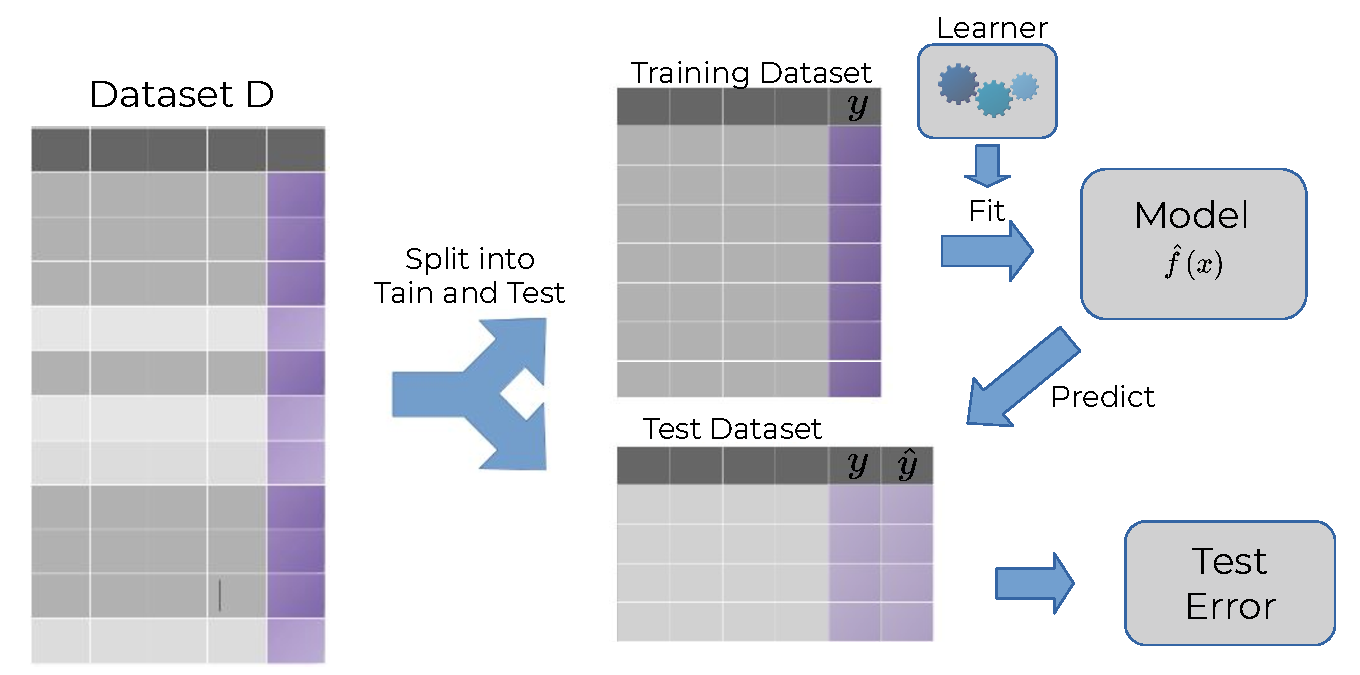
\includegraphics[width=0.8\textwidth, trim=270 0 0 0, clip]{figure_man/test_error.pdf}

\end{vbframe}



\begin{vbframe}{Test Error and Hold-Out Splitting}
\begin{itemize}
  \item Split data into 2 parts, e.g., 2/3 for training, 1/3 for testing
  \item Evaluate on data not used for model building
\end{itemize}

% FIGURE SOURCE: https://docs.google.com/drawings/d/1q7WN1_YKHedIPNySiZBEraLtTkHRX12Ej6M6ISbfMD0/edit?usp=sharing
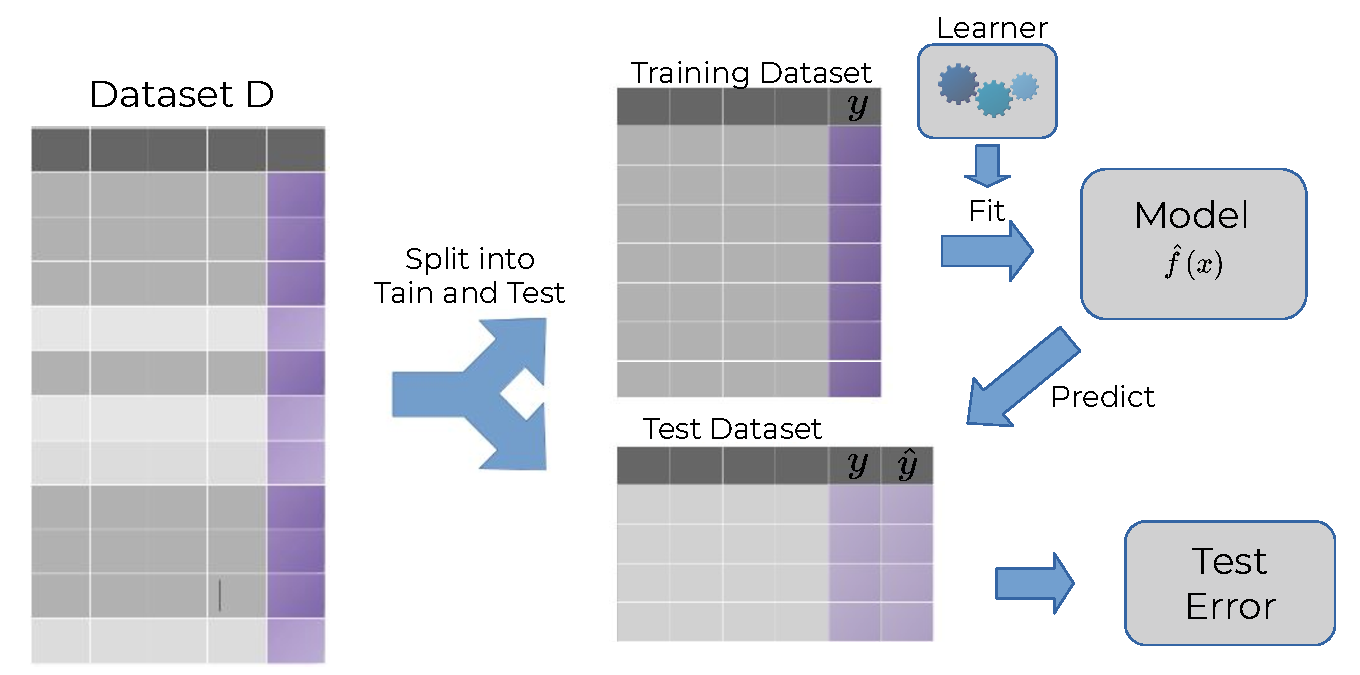
\includegraphics[width=\textwidth]{figure_man/test_error.pdf}

\end{vbframe}

\begin{vbframe}{Test Error}

Let's consider the following example:\\
Sample data from sinusoidal function
$0.5 + 0.4 \cdot \sin (2 \pi x) + \epsilon$\\
\lz
\begin{knitrout}\scriptsize
\definecolor{shadecolor}{rgb}{0.969, 0.969, 0.969}\color{fgcolor}

{\centering 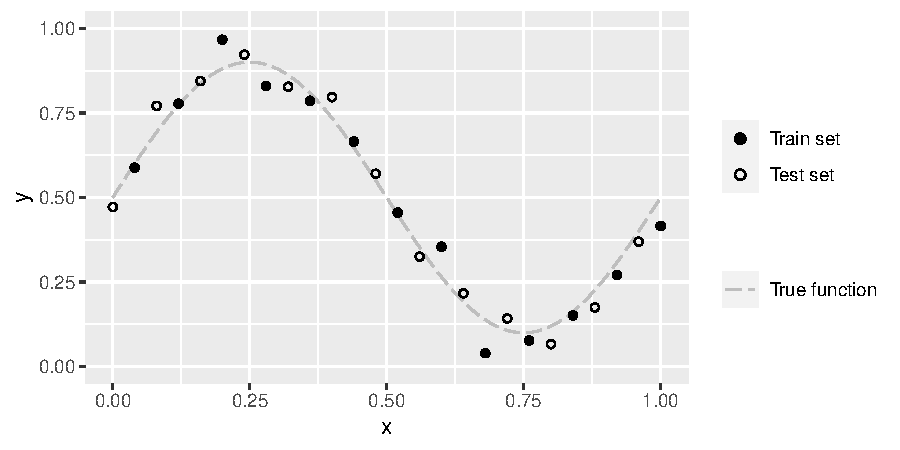
\includegraphics[width=0.8\textwidth]{figure/eval_test_1} 

}



\end{knitrout}
Try to approximate with a $d^{th}$-degree polynomial:
\[ \fxt = \theta_0 + \theta_1 x + \cdots + \theta_d x^d = \sum_{j = 0}^{d} \theta_j x^j\text{.} \]
\end{vbframe}


\begin{vbframe}{Test Error}
\begin{knitrout}\scriptsize
\definecolor{shadecolor}{rgb}{0.969, 0.969, 0.969}\color{fgcolor}

{\centering 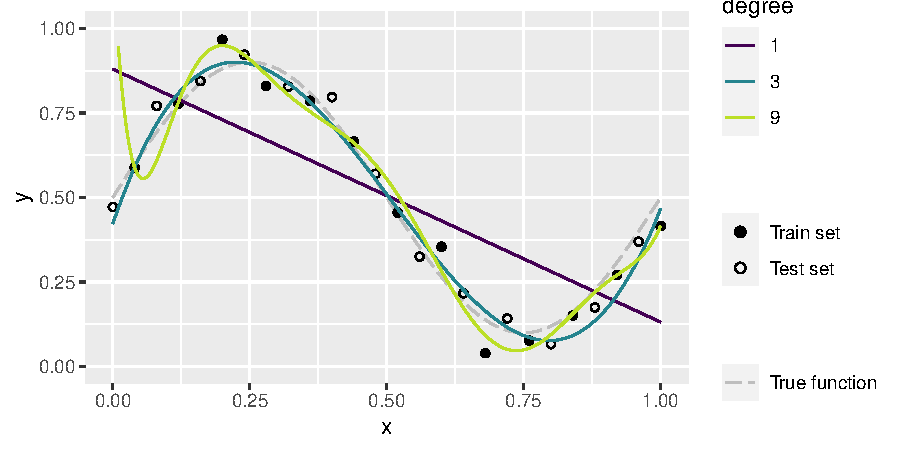
\includegraphics[width=0.95\textwidth]{figure/eval_test_2} 

}



\end{knitrout}

\begin{itemize}
\item d=1: MSE = 0.038: Clear underfitting
\item d=3: MSE = 0.002: Pretty OK
\item d=9: MSE = 0.046: Clear overfitting
\end{itemize}

\end{vbframe}


\begin{vbframe}{Test Error}
Plot evaluation measure for all polynomial degrees:
\begin{knitrout}\scriptsize
\definecolor{shadecolor}{rgb}{0.969, 0.969, 0.969}\color{fgcolor}

{\centering 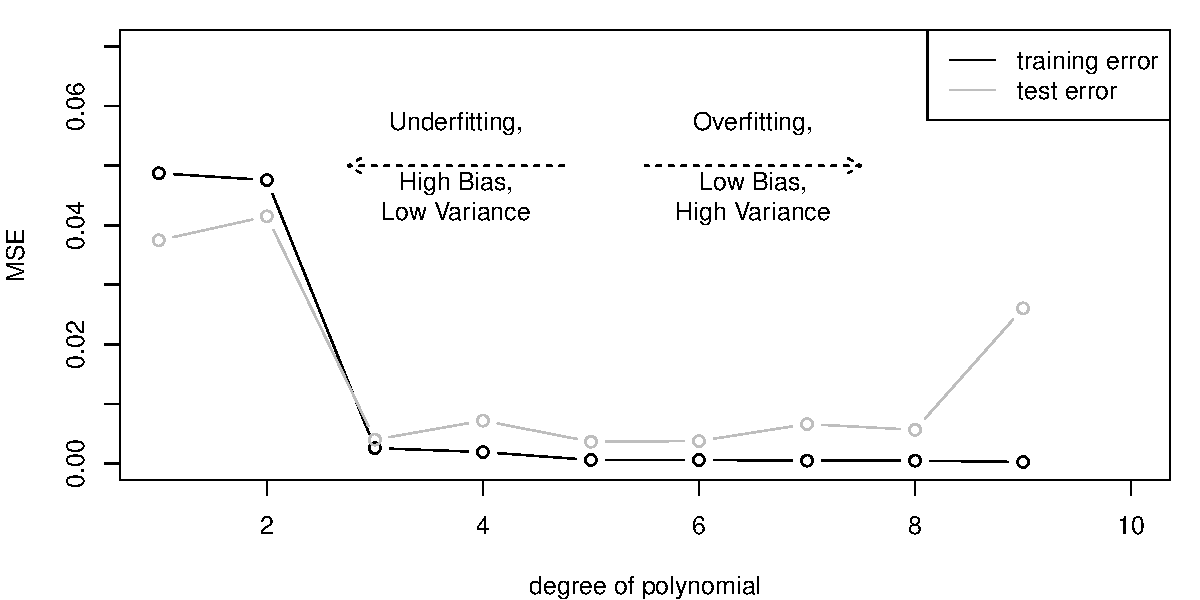
\includegraphics[width=0.9\textwidth]{figure/eval_test_3} 

}



\end{knitrout}

Increase model complexity (tendentially)
\begin{itemize}
\item decrease in training error\\
\item U-shape in test error\\ 
(first underfit, then overfit, sweet-spot in the middle)
\end{itemize}
\end{vbframe}

\begin{vbframe}{Test error Problems}
\begin{itemize}
  \item Test data has to be i.i.d. compared to training data.
  \item Bias-variance of hold-out:\\
  \begin{itemize}
    \item The smaller the training set, the worse the model $\rightarrow$ biased estimate.\\
    \item The smaller the test set, the higher the variance of the estimate.
  \end{itemize}   
  \item If the size of our initial, complete data set $\D$ is limited,
  single train-test splits can be problematic.
\end{itemize}
\end{vbframe}

\begin{vbframe}{Test error Problems}
A major point of confusion:
\begin{itemize}
\item In ML we are in a weird situation. We are usually given one data set. At the end of our model selection and evaluation process
we will likely fit one model on exactly that complete data set. As training error evaluation does not work,
we have nothing left to evaluate exactly that model.
\item Hold-out splitting (and resampling) are tools to estimate the future
performance. All of the models produced during that phase of evaluation are intermediate results.
% \item Keep that already in mind now, it will help to avoid confusion when we move on to cross-validation and nested cross-validation.
\end{itemize}
\end{vbframe}



% \begin{vbframe}{Test error Problems}
% Let's produce repeated 2/3 training, 1/3 testing splits on two ML tasks:\\ 
% a) iris ($n = 150, n_\text{test} \approx 50$) \\
% b) sonar ($n = 208, n_\text{test} \approx 70$).
% 
% \lz
% Plots below show the strong stochastic fluctuation of test errors\\
% (50 repeats).
% 
% <<echo=FALSE, fig.width = "\\textwidth", fig.height = 3, fig.align="center">>=
% my_ss = function(task) {
%   lrn = makeLearner("classif.naiveBayes")
%   r1 = subsample(lrn, task, iters = 50, show.info = FALSE)
%   return(r1$measures.test[,2])
% }
% err1 = my_ss(iris.task)
% err2 = my_ss(sonar.task)
% d = rbind(
%   data.frame(task = "iris", mce = err1),
%   data.frame(task = "sonar", mce = err2)
% )
% 
% ggplot(d, aes(x = mce)) + geom_histogram() + 
%     facet_wrap(vars(task), scales = "free_x") +
%     xlab("MCE")
% @
% \end{vbframe}
% 
% 

% 
% 
% % \begin{vbframe}{Training vs. test error}
% %   \vspace{-0.25cm}
% %   \begin{blocki}{The training error}
% %   \vspace{-0.25cm}
% %     \item is an over-optimistic (biased) estimator as the performance is measured on the same data the learned model was trained for
% %     \item decreases with smaller training set size as it is easier for the model to learn the underlying structure in the training set perfectly
% %     \item decreases with increasing model complexity as the model is able to learn more complex structures
% %   \end{blocki}
% %   \vspace{-0.25cm}
% %   \begin{blocki}{The test error}
% %   \vspace{-0.25cm}
% %   \item will typically decrease when the training set increases as the model generalizes better with more data (more data to learn)
% %   \item will have higher variance with decreasing test set size
% %   \item will have higher variance with increasing model complexity
% %   \end{blocki}
% % \end{vbframe}
% 
% 
% % \framebreak
% %
% % Visualize the perfomance estimator - and the MSE of the estimator - in relation to the true error rate.
% 
% % \begin{vbframe}{Bias-Variance of Hold-Out}
% % \begin{itemize}
% % \item If the size of our initial, complete data set $\D$ is limited,
% %   single train-test splits can be problematic.
% % \item The smaller our single test set is, the higher the variance
% %   of our estimated performance error (e.g., if we test on one observation, in the extreme case).
% %   But note that by just making the test set smaller, we do not introduce any bias,
% %   as we simply average losses on i.i.d. observations from $\Pxy$.
% % \item The smaller our training set becomes, the more pessimistic bias we introduce into the model.
% %   Note that if $|D| = n$, our aim is to estimate the performance of a model fitted
% %   on $n$ observations (as this is what we will do in the end). If we fit on less data during
% %   evaluation, our model will learn less, and perform worse. Very small training sets will also
% %   increase variance a bit.
% % \end{itemize}
% % \end{vbframe}
% 
% \begin{vbframe}{Bias-Variance of Hold-Out - Experiment}
% \begin{itemize}
% \item Data: simulate spiral data (sd = 0.1) 
% \item Learner: CART 
% \item Goal: estimate real performance of a model with $|\Dtrain| = 500$
% \item Get the "true" estimator by repeatedly sampling 500 observations from the simulator, fit the learner, then evaluate on $10^5$ observations
% \item Sample $\D$ with $|\D| = 500$ and analyze different split-rate $s \in \{0.05, 0.1, ..., 0.95\}$ for training with $|\Dtrain| = s \cdot 500$
% \item Estimate performance on $\Dtest$ with $|\Dtest| = 500 \cdot (1 - s)$
% \item Repeat the experiment for each split rate 50 times
% \end{itemize}
% 
% \framebreak
% 
% <<out.width="0.8\\textwidth", fig.height = 3, fig.width = 5>>=
% load("rsrc/holdout-biasvar.RData")
% ggd1 = reshape2::melt(res)
% colnames(ggd1) = c("split", "rep", "ssiter", "mmce")
% ggd1$split = as.factor(ggd1$split)
% ggd1$mse = (ggd1$mmce -  realperf)^2
% ggd1$type = "holdout"
% ggd1$ssiter = NULL
% mse1 = plyr::ddply(ggd1, "split", plyr::summarize, mse = mean(mse))
% mse1$type = "holdout"
% 
% ggd2 = plyr::ddply(ggd1, c("split", "rep"), plyr::summarize, mmce = mean(mmce))
% ggd2$mse = (ggd2$mmce -  realperf)^2
% ggd2$type = "subsampling"
% mse2 = plyr::ddply(ggd2, "split", plyr::summarize, mse = mean(mse))
% mse2$type = "subsampling"
% 
% ggd = rbind(ggd1, ggd2)
% gmse = rbind(mse1, mse2)
% ggd$type = as.factor(ggd$type)
% # ggd$split = as.numeric(as.character(ggd$split))
% gmse$split = as.numeric(as.character(gmse$split))
% gmse$type = as.factor(gmse$type)
% 
% ggplot(ggd[ggd$type == "holdout", ], aes(x = split, y = mmce)) +
%     geom_boxplot() + geom_hline(yintercept = realperf) + 
%     theme(axis.text.x = element_text(angle = 270, vjust = 0.5, hjust = 0)) +
%     ylab("MCE")
% 
% @
% 
% \begin{itemize}
% \item Pessimistic bias for small training sets
% \item Increased variance when test sets become smaller
% \end{itemize}
% 
% % \framebreak
% % 
% % \begin{itemize}
% %   \item We now plot the mean quadratic error between the true performance (line in 1st plot) and the hold-out values in each boxplot
% %   \item The split rate with the lowest MSE value produces the best estimator, which is pretty much 2/3 data for training
% %   \item NB: This is a single experiment and not a scientific study, but this rule-of-thump is also validated in larger studies
% % \end{itemize}
% % 
% % <<out.width="0.7\\textwidth", out.height="4cm">>=
% % ggplot(gmse[gmse$type == "holdout", ], aes(x = split, y = mse, col = type)) +
% %     geom_line() + scale_y_log10() + scale_x_continuous(breaks = gmse$split)
% %     theme(axis.text.x = element_text(angle = 270, vjust = 0.5, hjust = 0)) 
% % @
% 
% \end{vbframe}
\endlecture
\end{document}
